\icode{E-MM-SI-L3-261013-003}
如图所示，竖直光滑杆上穿有两个弹性小球\(A\)、\(B\)，其质量关系满足\(m_A \gg m_B\)，彼此间隔一小段距离，将两个小球从距底座高为\(h\)（\(h\)远大于小球半径）处由静止同时释放，所有碰撞时间极短且无机械能损失，则\(A\)、\(B\)第一次碰撞后\(B\)球上升的最大高度最接近\paren[]
	
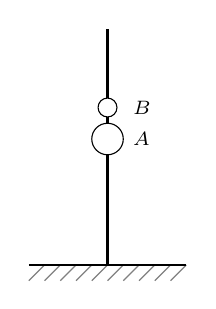
\begin{tikzpicture}[font=\scriptsize]
	\foreach \x in {-1,-.8,...,.8}
		\draw[gray] (\x,-.2)--++(.2,.2);
	\draw[thick] (-1,0)--(1,0) (0,0)--(0,3);
	\draw[fill=white] (0,1.6) circle(.2) (0,2) circle(.12);
	\node at(.2,1.6)[right]{\(A\)};
	\node at(.2,2)[right]{\(B\)}; 
\end{tikzpicture}
\begin{choices}
	\item\(4h\)
	\item\(6h\)
	\item\(8h\)
	\item\(9h\)
\end{choices}
\begin{answer}
    D\qquad 提示：\(v_1^{\prime} = \frac{(m_1 - m_2)v_1 + 2m_2v_2}{m_1 + m_2} = \frac{(\frac{m_1}{m_2} - 1)v_1 + 2v_2}{\frac{m_1}{m_2} + 1}\)，当\(m_1\gg m_2\)时，\(\frac{m_1}{m_2}\to 0\)，\(v_1 = - v_1 + 2v_2\)
\end{answer}